\documentclass{article}
\usepackage{indentfirst}
\usepackage{lmodern}
\usepackage[utf8]{inputenc}
\usepackage[T1]{fontenc}
\usepackage[ngerman]{babel}
\usepackage{amssymb,amstext,amsmath}
\usepackage{graphicx}
\usepackage{dsfont}
\usepackage{amsfonts}
\usepackage{graphics}
\usepackage{float}
\usepackage{cite}
\usepackage{url}
 
\title{Fabry-Perot-Etalon}
\author{Alexander Heinisch, Dominik Wille}
\begin{document}
\maketitle
\vspace{13cm}
\noindent
\begin{center}
\begin{tabular}{r l}
Tutor & Diana Prychnenky  \\
Durchführung & 08. Mai 2013 \\

E-Mail Dominik & dominik.wille@fu-berlin.de \\
E-Mail Alexander & matthias.heinisch@gmx.de \\
\end{tabular}
\end{center}

\newpage
\tableofcontents
\newpage

\section{Ziele des Versuchs}
Experimentelle Einführung in das {\sc Fabry-Perot-Interferometer} als wichtiges Bauteil hochauflößender Spektralapparate und der Lasertechnik \\

\section{Physikalische Grundlagen}

\subsection{Vielstrahleninterferenz}
Bei der Beugung von Licht an einem Einfach- oder einem Doppelspalt entseht ein Interferenzmuster mit breiten Hauptmaxima und relativ dünnen Minima. Diese werden durch den Gangunterschied der Elementarwellen und die darauf folgende konstruktive bzw. destruktive Interferenz, hervorgerufen. Im Gegensatz dazu steht die Beugung des Lichts an einem optischen Gitter. Aufgrund der periodischen Struktur entstehen Vielfachinterferenzen mit sehr schmalen Interferenzmaxima und breiten Minima. Dies ermöglicht bei verschiedenen messtechnischen und spektroskopischen Anwendungen eine hohe Auflösung. 

\subsection{Fabry-Perot-Etalon}
Ein Fabry-Perot-Etalon (oder auch Fabry-Perlot-Interferrometer) ist ein optischer Resonator. Er besteht aus zwei parallelen, teilverspiegelten Flächen \(\ (G_{1} \) und \(\ G_{2} \)), zwischen denen eine einfallende ebene Welle \(\ (E_{e} \)) eine ''Zick-Zack-Reflexion'' erfährt. Da zwischen den Grenazflächen ein optisches Medium eingesperrt ist (z.b. Luft), wird der Lichtstrahl in kohärente Teilwellen \(\ (E_{i} \)) aufgespalten, die miteinander interferieren und eine auslaufende Welle \(\ (E_{a} \)) bildet. Den Gangunterschied berechnen wir mit

\begin{equation}
\label{1}
\delta = \overline{AC} + \overline{CD} - \overline{AB}= \frac{2d}{cos \alpha}- \frac {2d \cdot sin^2 \alpha}{cos \alpha} =2d\cdot cos \alpha
\end{equation}\\

Wobei A, B und C nacheinander die Punkte der Reflexion an den Spiegeln sind, \(\alpha \) ist der Einfallswinkel und d der Plattenabstand. Daraus folgt, dass sich der Gangunterschied verkleinert, wenn \(\alpha \) größer wird.

Des Weiteren können wir einen Gangunterschied durch Phasensprünge bei den Reflexionen vernachlässigen, da er bei Transmissionen einem ganzzahligen Vielfachen der Wellenlänge entspricht. Daraus folgt für transmittiertes Licht

\begin{equation}
\label{2}
\delta = 2 \cdot d \cdot cos \alpha = z \cdot \lambda \ \ \ mit\ z=1,2,3...
\end{equation}\\

Somit ist ersichtlich, dass nur dann Interfereinsmaxima entstehen, wenn \(\alpha \) oder \(\lambda \) Gl. \eqref{2} erfüllen.
\begin{figure}[htbp]
\centering
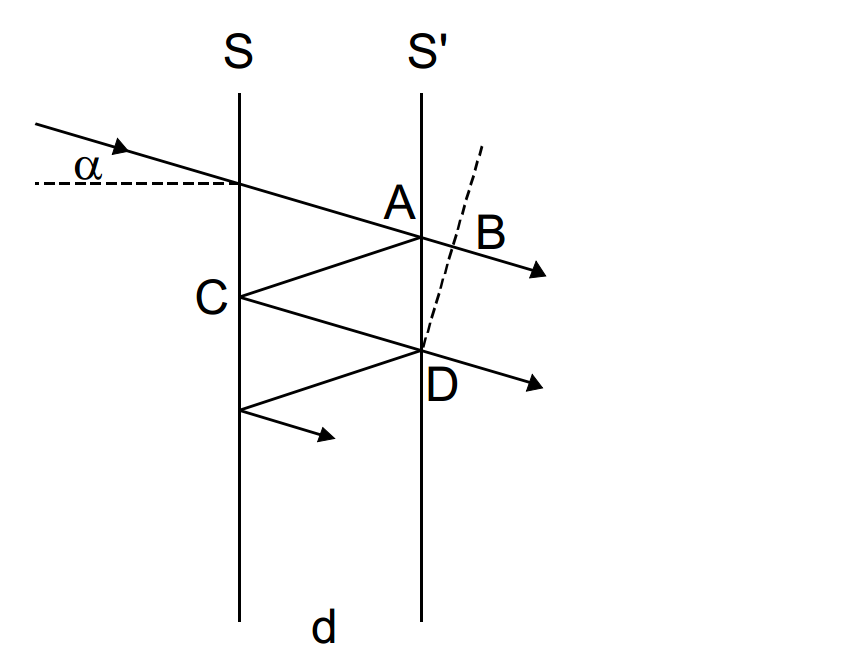
\includegraphics[scale=0.3]{FAP1.png}
\begin{center}
\caption{Aufbau Fabry-Perlot-Interferometer [GP 2 Skript]}
\end{center}
\end{figure}

Die Phasengröße \(\phi \) bezeichnet den Gangunterschied in Einheiten der Wellenlänge, dich sich wie Folgt berechnet

\begin{equation}
\label{3}
\phi = \frac {\delta}{\lambda}
\end{equation}\\

Man nennt die ganzzahligen Werte Z von \(\phi \) Interferenzordnung der Maxima.

\subsection{Freier Spektralbereich}
In einem Dispersionsgebiet, kann man die ungestörten Wellenlängen eines Spektralapparats untersuchen. Als Bedingung für Interferenz gilt immer noch \eqref{2}, wobei man hier zwischen zwei Fälle unterscheidet. Entweder unterscheiden sich zwei benachbarte Maxima durch einen Ordnungsunterschied \(\Delta z =1 \) bei gleicher Wellenlänge, oder durch eine Wellenlängendifferenz \(\Delta \lambda \) bei gleicher Ordnung.
Somit wird aus \eqref{2} 

\begin{equation}
\label{4}
(z+1) \lambda=z( \lambda + \Delta \lambda)
\end{equation}
\vspace{0,25cm}

Daraus folgt für den freuen Spektralbereich des Etalons

\begin{equation}
\label{5}
\Delta \lambda = \frac {\lambda}{z} \  \ oder \ \ \frac {\Delta \lambda}{\lambda} = \frac {1}{z}
\end{equation}\\

Will man also ein nahezu monochromatisches Licht untersuchen oder eine Feinuntersuchung enger Wellenlängenbereiche durchführen, verwendet man den {\sc Fabry-Perot-Etalon}, welcher wegen seinem kleinen Dispersionsgebiet bei großen z besonders gut geeignet ist.

\subsection{Fabry-Perot-Spektrometer}
Wollen wir nun den Etalon als Spektrometer verwenden, müssen wir ihn mit divergentem Licht beleuchten, von dem unter einem bestimmten Einfallswinkel nur genau eine Farbe passieren kann. Dabei werden durch die Rotationssymmetrie der optischen Anordnung in der Brennebene der Linse konzentrische Ringe gleicher Neigung (Haudingersche Ringe) abgebildet. Nun setzten wir für den Neigungswinkel \(\alpha\) und \(cos\ \alpha \) näherungsweise

\begin{equation}
\label{6}
\alpha = \frac {r}{f} \ \ und \ \ cos \alpha = 1- \frac {1}{2} \alpha ^2
\end{equation}\\

für die Brennweite f der Linse und Radius r des Ringes, folgt für Gl.\eqref{2}

\begin{equation}
\label{7}
z \approx \frac {2d}{\lambda} \left [ 1-\frac {r^2}{2f^2} \right ]
\end{equation}
lösen wir nun zuerst die Klammern auf, stellen die Gleichung nach\(\ \left(\frac{2d}{\lambda }\right)\) um und klammern anschließend z wieder aus, erhalten wir:
\begin{equation}
\frac {2d}{\lambda} \approx z \left [1+ \frac {r^2}{2f^2} \right ]
\end{equation}\\

Um nun z aus den Gleichungen zu eliminieren, misst man bei bekannten Größen \(\ f, \lambda \) und \(\ d \) mindestens zwei Radien des Ringsystems und erhält für den Grenzflächenabstand

\begin{equation}
\label{8}
d = i \frac {\lambda f^2}{r_{i}^2 - r_{0}^2}
\end{equation}

mit i = 1,2,3,... dem Index des Ringes.
Sind \(\ d \) und \(\ z \) nicht bekannt, kann man die Wellenlänge \(\lambda \) und \(\lambda ' = \lambda + \Delta \lambda \) einer Ordnung mit den Radien \(\ r \) und \(\ r' \) aus

\begin{equation}
\label{9}
\Delta \lambda \approx \frac {\lambda}{2f^2} (r^2 - r'^2)
\end{equation}\\

berechnen. Da die Ordnung eliminiert wurde, lässt die Genauigkeit nach, was zur Folge hat, dass man die Größen \(\ d \) und \(\ z \) möglichst genau bestimmt werden.\\

\subsection{Auflösungsvermögen des Fabry-Perot-Etalon} 
Will man die genaue Intensitätsverteilung um ein Interferenzmaximum in Abhängigkeit der Phasengröße \(\phi \) bestimmen, benötigt man die {\sc Airy-Formel}

\begin{equation}
\label{10}
\frac {I}{I_{0}} = \left [ \frac {T}{1-R} \right ]^2 \cdot \frac {1}{1+ \frac {4R}{(1-R)^2} \cdot sin^2 \phi \pi}
\end{equation}

mit dem Transmissionsgrad T und Reflexionsgrad R der Platten. Dafür folgt für die Halbwertsbreite \(\ 2 \Delta z \) der Interferenzmaxima näherungsweise für kleine Winkel

\begin{equation}
\label{11}
2 \Delta z= \frac {1-R}{\pi \sqrt {R}}
\end{equation}\\

\section{Aufgaben}
\subsection{Aufgabe 1}
Aufbau und Justierung der Apparatur.
\subsection{Aufgabe 2}
Bestimmung des Plattenabstandes eines {\sc  Fabry-Perot-Etalon} mit der roten 643,9-nm-Linie von Cadmium und Berechnung der (ungefähren) Interferenzordnung.
\subsection{Aufgabe 3}
Relative Bestimmung der Wellenlängen der grünen und der dunkelblauen Linie des Cadmium-Spektrums.
\subsection{Aufgabe 4}
Abschätzung der Linienbreite der Interferenzmaxima für die rote Linie und Vergleich mit der erwarteten instrumentellen Linienbreite.

\newpage

\section{Auswertung}
\subsection{Aufgabe 1}
Der Aufbau der Apparatur war an sich relativ trivial, da die meisten Linsen etc. schon auf der Schiene befestigt waren. An sich mussten wir nur noch die passende Lampe finden und alle Linsen in die passenden Abständen schieben. Als nächstes mussten wir alle Linsen und den Fabry-Perlot-Etalon in die richtige Höhe bringen, damit der Strahlengang der Cadmium-Lampe ungehindert im Okular ankam. Als wir alle Fehler korrigiert hatten, mussten wir nur noch den Filter in die Halterung einsetzen und das Fadenkreuz im Okular auf den von innen zehnten Ring des Interferenzmusters einstellen.
Der Aufbau sah letztendlich wie folgt aus:

\begin{figure}[H]
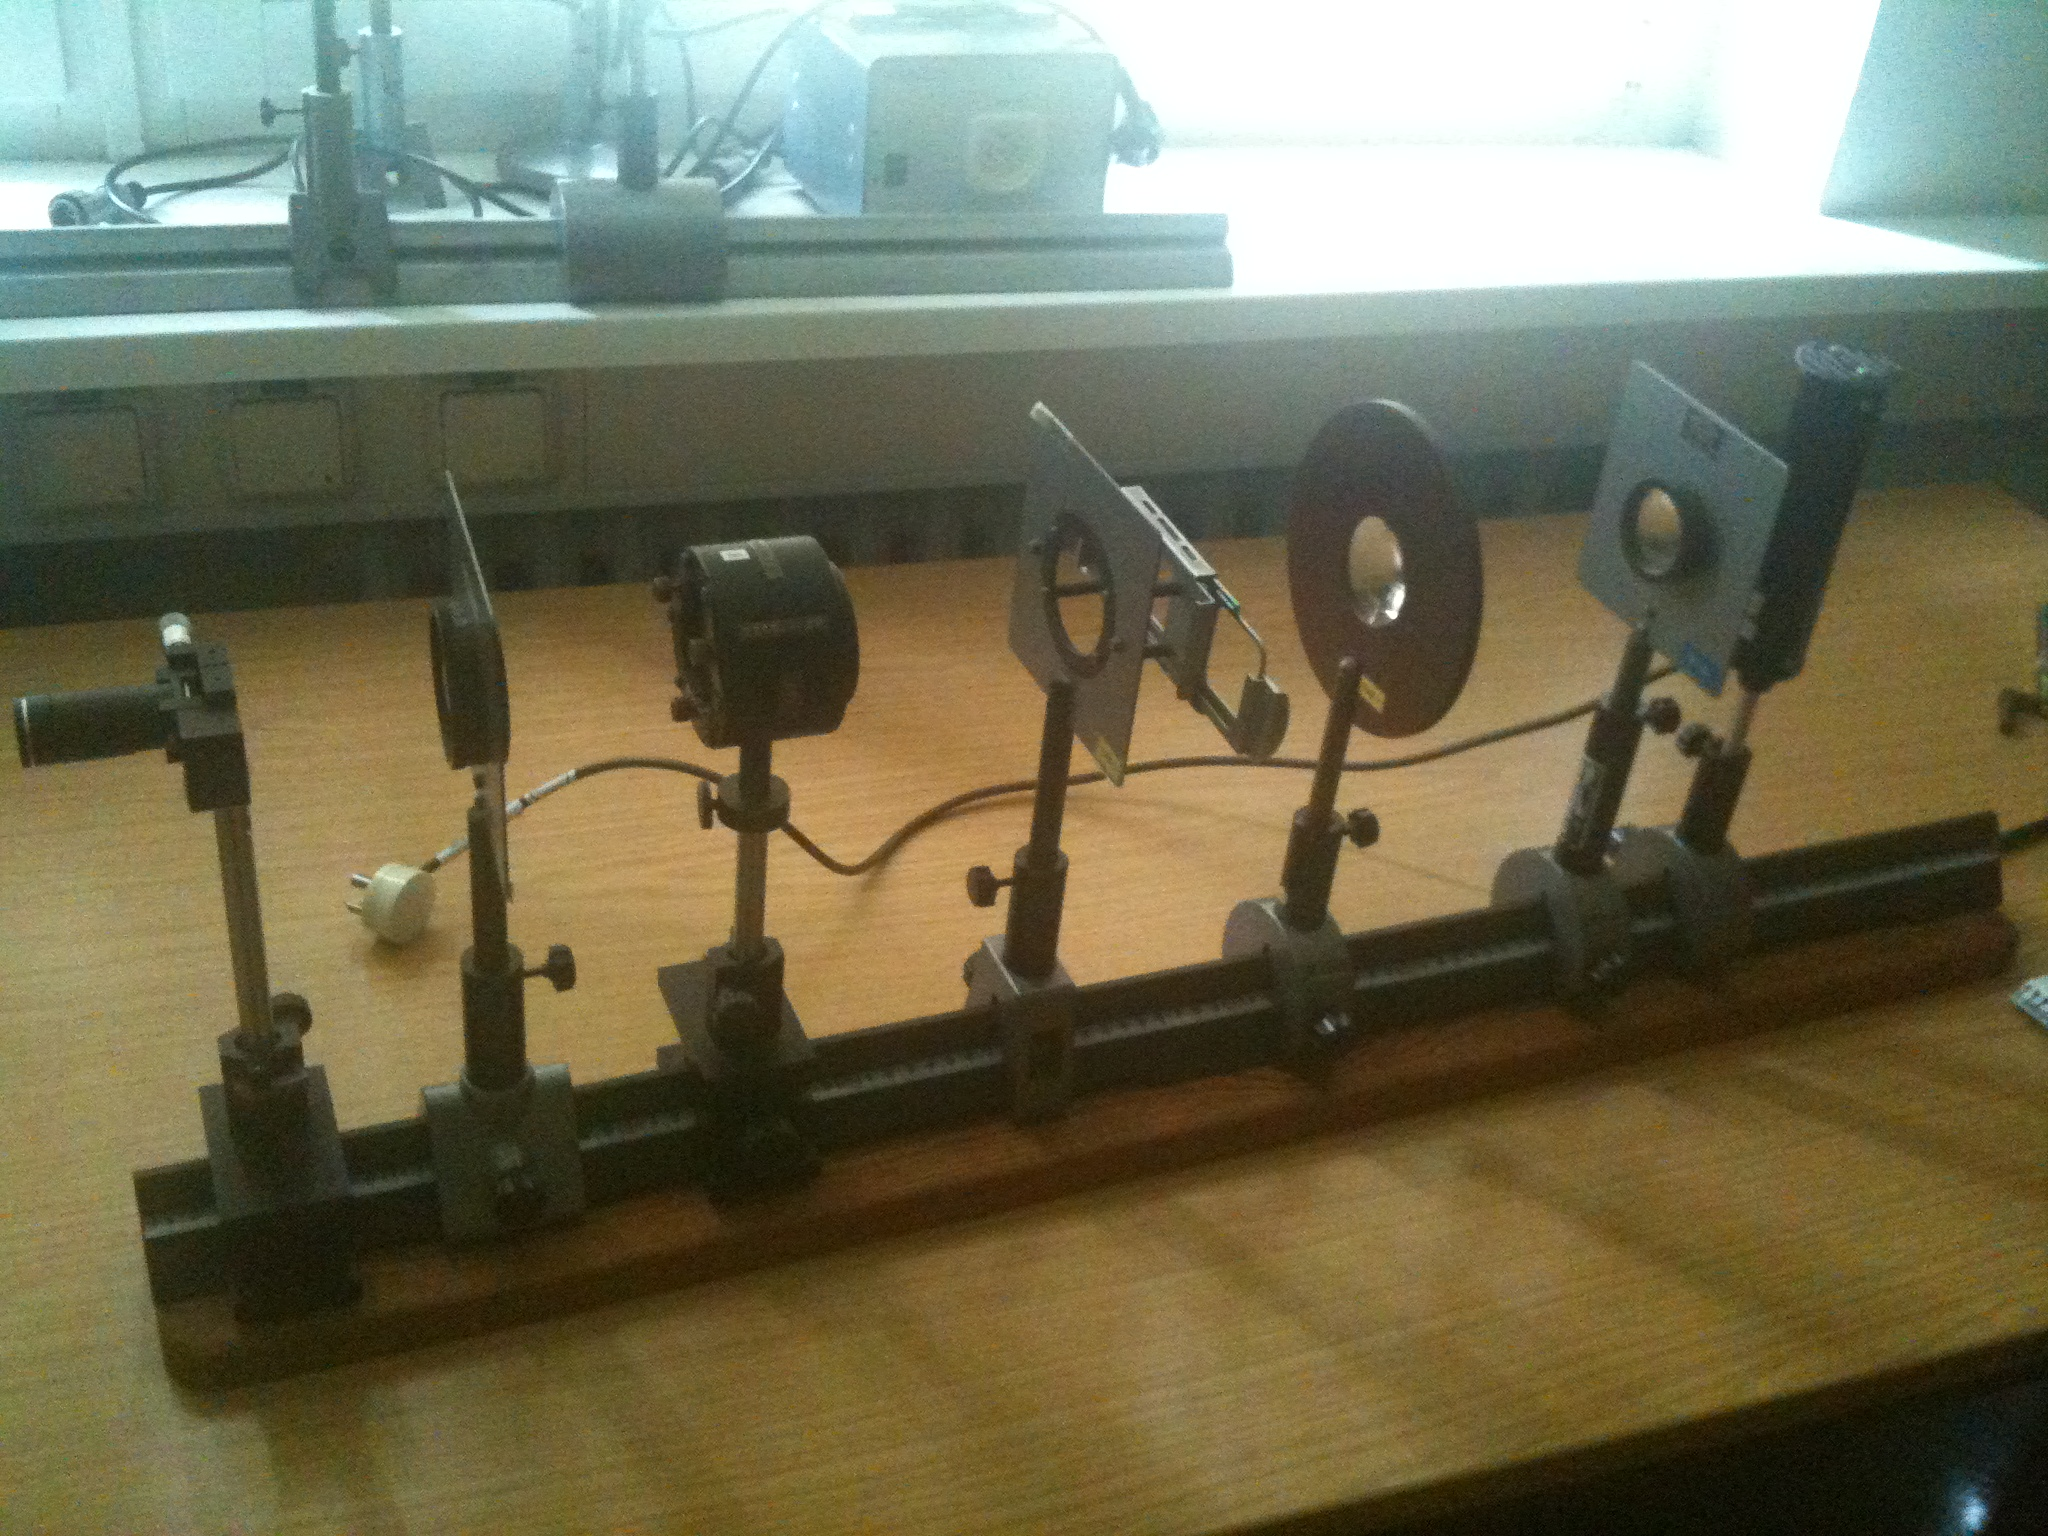
\includegraphics[scale=0.2]{IMG_0021}
\caption{Aufbau, von links nach rechts: Okular, 1. Konvexlinse (f=), Etalon, Farbfilter, 2. Konvexlinse (f=), 3. Konvexlinse (f=), Cadmium-Lampe}
\end{figure}

\subsection{Aufgabe 2}

\subsection{Aufgabe 3}

\section{Aufgabe 4}
\subsection{Auswertung}
Nun sollen wir die Linienbreite schätzen, wozu wir den kleinsten erkennbaren Ring benutzten 
\\

\begin{tabular}{l|l|l|l|l}
 & \multicolumn{2}{c|}{\textbf{Ringabmessung rechts [mm]}} & \multicolumn{2}{c}{\textbf{Ringabmessung links [mm]}} \\
Ring i & & & & \\
		& Position innen & Position außen & Position innen & Position außen\\	
\hline
 & $9.48\pm 0.17$ & $9.15\pm 0.17$ & $12.01\pm 0.19$ & $12.39\pm 0.19$ \\
1 & & & & \\
& Radius innen [mm] & Radius außen [mm] & Radius gemittelt [mm] &\\ \hline
& & &  \\
1 & $1.27\pm 0.13$ & $1.62\pm 0.13$ & $1.45\pm 0.19$\\
\end{tabular}\\
\begin{center}
\it Tab. 4.1: innerstes vermessene Maxima\\
\end{center}

Die Linienbreite L bestimmen wir nun über die Gl.$\eqref{9}$

\begin{equation}\notag
L\approx \Delta \lambda \approx \frac {\lambda}{2f^2} (r^2 - r'^2)
\end{equation}\\
Der Fehler errechnet sich aus der Gauß'schen Fehlerfortpflanzung:

\begin{equation}
\Delta L=\sqrt{\frac{(r_{a}^2-r_{i}^2)^2\Delta \lambda^2}{4f^4}+\frac{(r_{a}^2-r_{i}^2)^2\Delta L^2\lambda^2}{f^6}+\frac{r_{a}^2\Delta r_{a}^2\lambda^2}{f^4}+\frac{r_{i}^2\Delta r_{i}^2\lambda^2}{f^4}}
\end{equation}
Daraus folgt für $L=(33.57\pm 2)pm$\\
\\
Um die Größe z zu berechnen, benutzten wir Gl.\(\eqref{7}\) mit:
\begin{equation}\notag
z\approx \frac{2d}{\lambda}\left[1-\frac{r^2}{2f^2}\right]\approx \frac{2\cdot 3,66\cdot 10^{-3}}{643,3\cdot 10^{-9}}\left[1-\frac{(4,018\cdot 10^{-3})^2}{2\cdot (10\cdot10^{-2})^2}\right]\approx 11359,1
\end{equation}

Um nun den theoretischen Wert zu berechnen, benutzen wir die Airy-Formel für näherungsweise kleine Winkel Gl.$\eqref{11}$

\begin{equation}\notag
L_{theo}=\frac{2 \Delta z\cdot \lambda}{z}=\frac{\frac {1-R}{\pi \sqrt {R}}\lambda}{z} 
\end{equation}\\
\\
Und für den Fehler:

\begin{equation}\notag
\begin{split}
\Delta L_{theo}=\sqrt{\left(\frac{\partial L_{theo}}{\partial R}\cdot \Delta R\right)^2+\left(\frac{\partial L_{theo}}{\partial z}\cdot \Delta z\right)^2}\\
\Delta L_{theo}=\sqrt{\frac{(1-R)^2\cdot\Delta z^2\lambda^2}{\pi^2\cdot R\cdot z^4}+\Delta R\left(\frac{-(1-R)\lambda}{2\pi R^{\frac{3}{2}}\cdot z}-\frac{\lambda}{\pi \cdot \sqrt{R}\cdot z}\right)^2}
\end{split}
\end{equation}

Mit $R=80\%$, $z=11359,1$ und $\Delta R=5$ (was wir nicht genau kannten und so festlegten) folgt für $L=(4.1\pm 1.3)pm$

\subsection{Fazit}
Die große Abweichung zwischen dem theoretischen Wert L=(4.1$\pm$1.3)pm und dem berechneten Wert L=(33$\pm$2)pm liegt wahrscheinlich größtenteils an der subjektiven Wahrnehmung des menschlichen Auges, da es, wie bei vielen optischen Versuchen, mit der Zeit immer anstrengender wird und die Konzentration nachlässt. Weitere Fehlerquellen sind das Auflösungsvermögen des Versuchsaufbaus,sowie die quantenmechanischen Effekte der Dopplerverbreiterung (Effekte, welche durch die thermische Bewegung der Atome auftreten) und die Druckverbreiterung (welche durch die verringerte Lebensdauer der Cadmium-Atome durch Stöße verursacht wird).
Noch weitere Ringe zu messen hätte die Auswertung genauer gemacht, aber schon die zehnte Ordnung war recht schwer zu erkennen.

\section{Fazit}
\section{Qellenangabe}
GPII-Skript\\
\end{document}